\chapter{Experiment Results}
\label{chapter6}
\hspace*{6mm}For checking and validating the proposed method, we set up experiments from technical and pre-clinical perspective. In technical perspective, admittance control, force-guided alignment, and file feedrate control were conducted and verified. On the other hand, in pre-clinical evaluation, acrylic root models before and after performing endodontic treatment with DentiBot were also compared in this chapter. 
\section{Experimental Setup}
\subsubsection{Software and Firmware Setup}
\hspace*{6mm}To control and communicate with all devices in low latency, low jitter, and high speed, a communication protocol - Ethernet for Control Automation Technology (EtherCAT) and a real-time oprating system (RTOS) are interfaced. EtherCAT is constructed on EtherNET and utilizes "processing on the fly" technology. Therefore, it provide a short cycle time (less than 100 \textmu s) and a low jitter \cite{web5}. Besides, EhterCAT supports every types of network topologies such as star, ring, daisy chain, and so on.	 All devices are connected in Daisy-chain with EtherCAT as shown in Fig \ref{fig:EtherCAT}. Graph user interface and fundamental framework are constructed to reduce and eliminate future developing problems as shown in Fig \ref{fig:GUI}.

\begin{figure}[htbp]
\begin{center}
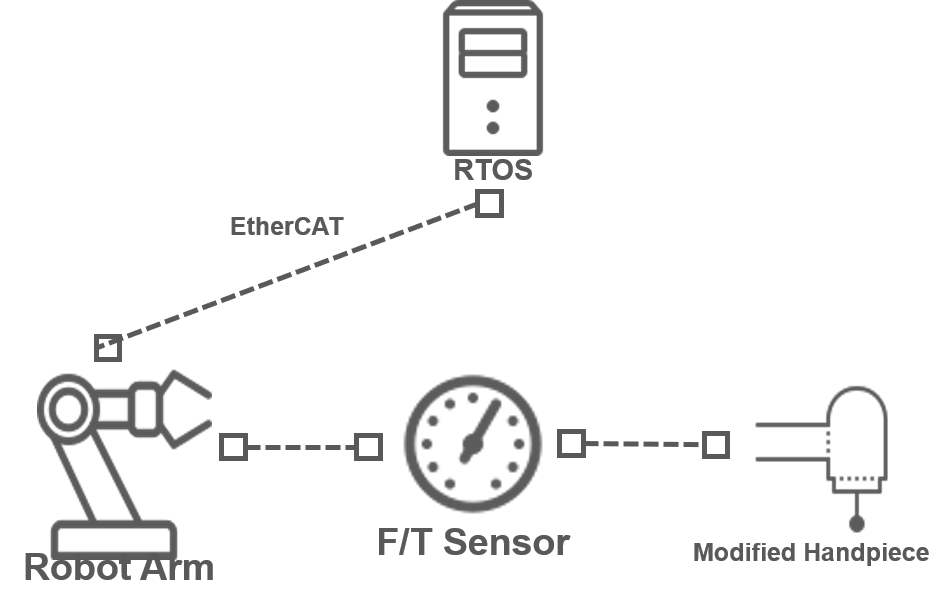
\includegraphics[width=0.7\linewidth]{Images/EtherCAT.png}
\caption{Communication protocol -- EtherCAT. Master device is RT-target and slave devices are robot arm, F/T sensor and modified handpiece.}
\end{center}
\end{figure}
\label{fig:EtherCAT}
\begin{figure}[htbp]
\begin{center}
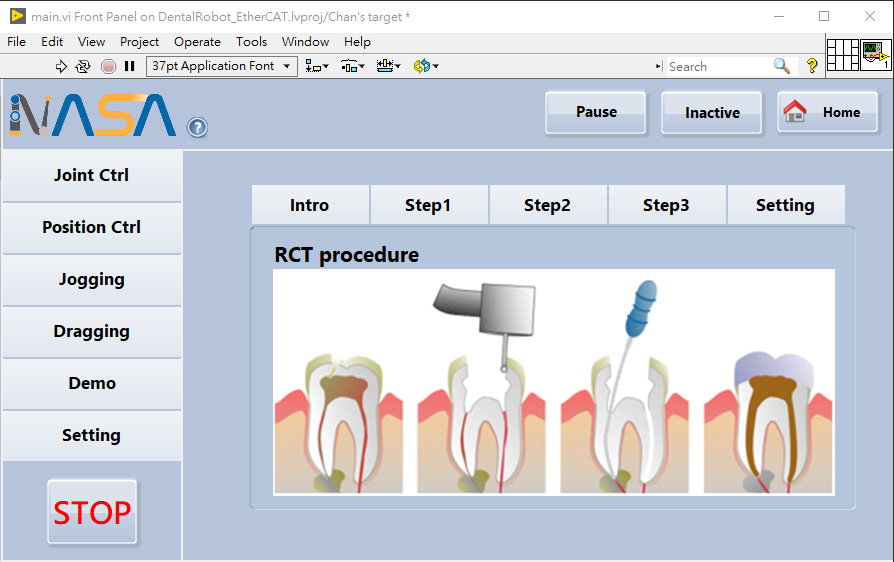
\includegraphics[width=1\linewidth]{Images/GUI.png}
\caption{Graph user interface with LabVIEW 2018}
\label{fig:GUI}
\end{center}
\end{figure}

\par
\subsubsection{Hardware Setup}
\hspace*{6mm}In Fig \ref{fig:system}, a motion capture system was incorporated to obtain the position information \cite{web8}. There are four cameras with high resolution sensor around the robot. It can capture LEDs and calculate their Cartesian position for $960$ frames per second and its resolution is around $1$ mm. Moreover, a Stewart Platform on which a root acrylic model is mounted was set up to simulate a small patient moving. To record the handpiece and root positions, a LED marker is located on the driller and other three LED markers forming a equilateral triangle are seated on the Stewart platform and. Therefore, the handpiece position is directly obtained and the root position is calculated as following equation
\begin{equation*}
\begin{split}
p_{root} = \frac{p_{1} + p_{2} + p_{3}}{3}
\end{split}
\end{equation*}
where $p_{root}$ denotes the root position and $p_{i}$ denote the positions of LEDs obtained from the motion capture system. 
\par
Note that there is a original vertical distance between the root and handpiece in this setup and an error come from inaccurate 3-D print support used to stick three LEDs. Besides, once the motion capture system captures a LED with less than three cameras, the position information will be incorrect. 
\begin{figure}[htbp]
\begin{center}
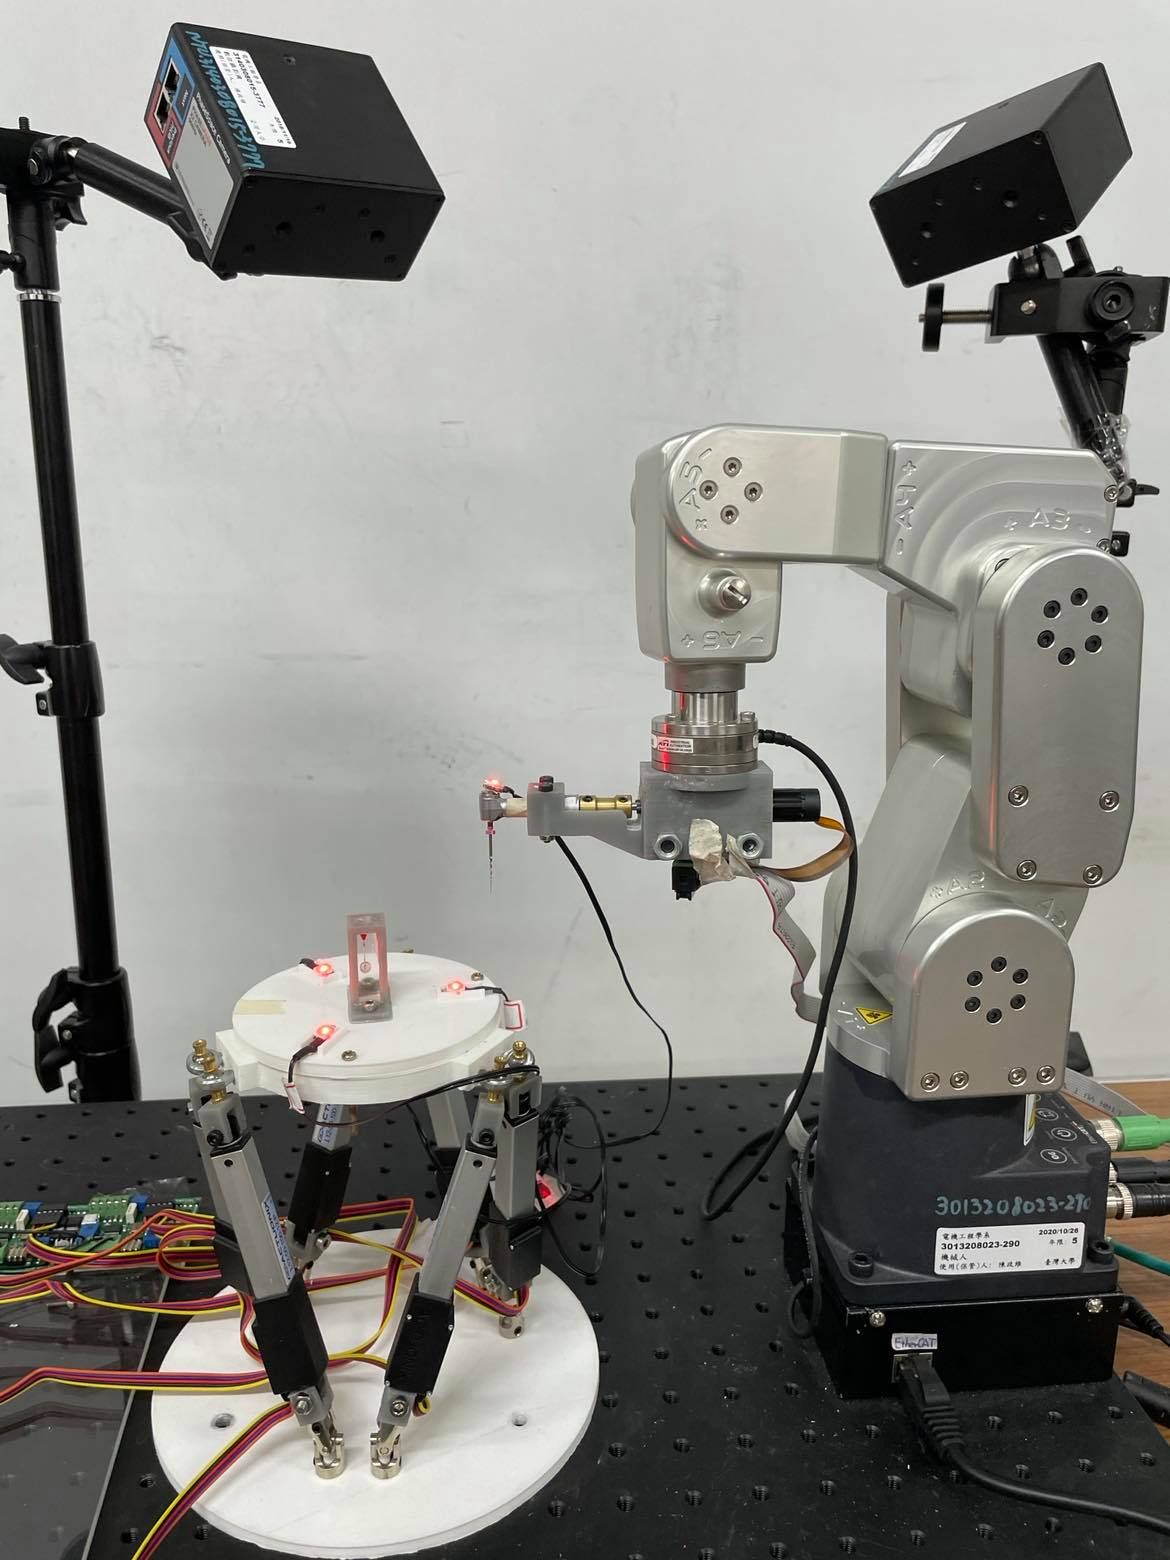
\includegraphics[width=0.7\linewidth]{Images/System.jpg}
\caption{Experimental setup with Dentibot, a motion capture system, and a Stewart platform}
\label{fig:system}
\end{center}
\end{figure}
\par
The specifications of the hardware and software environment set in the experiments are listed in Table \ref{tab:exp_specification}. The detail specifications of the robot arm and F/T sensor are shown in Table \ref{tab:meca_specification} and Table \ref{tab:mini40_specification}.

\begin{table}[htbp]
\centering
\tabcolsep=20pt
\arrayrulewidth=1pt
\caption{Specifications of the hardware and software environments}
\label{tab:exp_specification}
\par
\begin{tabular}{|c|c|} 
\hline
\rowcolor{lightgray!40}Item						&Specification				\\	\hline
Development Environment							&LabVIEW 2018					\\	\hline
\multirow{2}{*}{Real-Time Operating System}		&National Instrument-RT target	\\
												&CPU: Intel Core 8				\\	\hline
Communication Protocol							&EtherCAT						\\	\hline
Robot Arm										&Mecademic-Meca500				\\	\hline
F/T Sensor										&ATI-Mini40						\\	\hline
\multirow{2}{*}{Handpiece Motor}							&Maxon - servo motor				\\
												&Gear ratio: 67					\\	\hline
\multirow{2}{*}{Motion Capture System}			&PhaseSpace-Impulse X2E 		\\
												&Resolution: 1mm				\\	\hline
Stewart Platform								&Actuoanix - Linear Actuator				\\	
\hline
\end{tabular}
\end{table}

\begin{table}[htbp]
\centering
\tabcolsep=18pt
\arrayrulewidth=1pt
\caption{Technical specifications of the robot arm - meca500}
\label{tab:meca_specification}
\par
\begin{tabular}{|>{\columncolor{lightgray!20}}c|l|} 
\hline
Payload						&$0.5$ kg					\\	\hline
Repeatability				&$0.005$ mm					\\	\hline
Reach (at wrist center)		&$260$ mm	\\ \hline
Total weight				&$4.5$ kg						\\	\hline
\multirow{6}{*}{}Joint range&joint 1: $-175^\text{o}$ to $+175^\text{o}$				\\	
							&joint 2: $-70^\text{o}$ to $+90^\text{o}$				\\	
							&joint 3: $-135^\text{o}$ to $+70^\text{o}$				\\	
							&joint 4: $-170^\text{o}$ to $+170^\text{o}$				\\	
							&joint 5: $-115^\text{o}$ to $+115^\text{o}$				\\	
							&joint 6: $\pm 100$ revolutions				\\	\hline
Speed of joints 1–6 &${150, 150, 180, 300, 300, 500}$ $^\text{o}\text{/s}$				\\	\hline
Brakes 				&On joints 1, 2 and 3				\\	\hline
Robot mounting 		&Any orientation				\\	\hline
Safety module		&Category 3, PL d				\\	\hline
Power supply 		&90-264 VAC, 50-60 Hz (in) / 24 VDC (out)				\\	\hline
Communication 		&TCP/IP, EtherCAT, Ethernet/IP				\\	\hline
Controller 			&Embedded in robot base				\\	\hline
Protection rating 	&IP 40								\\	
\hline
\end{tabular}
\end{table}

\begin{table}[htbp]
\centering
\tabcolsep=10pt
\arrayrulewidth=1pt
\caption{Technical specifications of the F/T sensor - mini40}
\label{tab:mini40_specification}
\par
\begin{tabular}{|>{\columncolor{lightgray!20}}c|l|} 
\hline
Weight										&0.0499 kg	\\  \hline
Diameter									&40 mm  	\\ 	\hline
Height										&12.2 mm 	\\	\hline
\multirow{4}{*}{}Sensing range					&Fx,Fy: 20 N\\
											&Fz: 60 N\\
											&Tx,Ty: 1 Nm\\	
											&Tz: 1 Nm\\	\hline
\multirow{4}{*}{}Resolution						&Fx,Fy: 1/100 N	\\
											&Fz: 1/50 N\\
											&Tx,Ty: 1/4000 Nm\\	
											&Tz: 1/4000 Nm\\	\hline										
\multirow{4}{*}{}Single-axis overload 			&Fxy: ±810 N  \\	
											&Fz	±2400 N  \\
											&Txy	±19 Nm  \\
											&Tz	±20 Nm  \\ \hline
\multirow{4}{*}{}Stiffness (calculated)   		&X-axis \& Y-axis forces (Kx, Ky): 1.1x107 N/m   \\	
											&Z-axis force (Kz): 2.0x107 N/m   \\	
											&X-axis \& Y-axis torque (Ktx, Kty): 2.8x103 Nm/rad   \\	
											&Z-axis torque (Ktz): 4.0x103 Nm/rad   \\	 \hline
\multirow{2}{*}{}Resonant Frequency 			&Fx, Fy, Tz: 3200 Hz  \\
											&Fz, Tx, Ty: 4900 Hz  \\
\hline
\end{tabular}
\end{table}

\newpage
\section{Force-Guided Alignment}
\hspace*{6mm}In order to prove the validation of force-guided alignment, we set up three experiments with different scenarios. The aim of these experiments was for validating whether it was possible that the DentiBot inserted an endodontic file into a small root and confronted a patient moving at the same time. Therefore, three experiment were designed with more and more functions listed below and shown in Fig \ref{fig:exp_motion planning}.

\begin{figure}[htbp]
\begin{center}
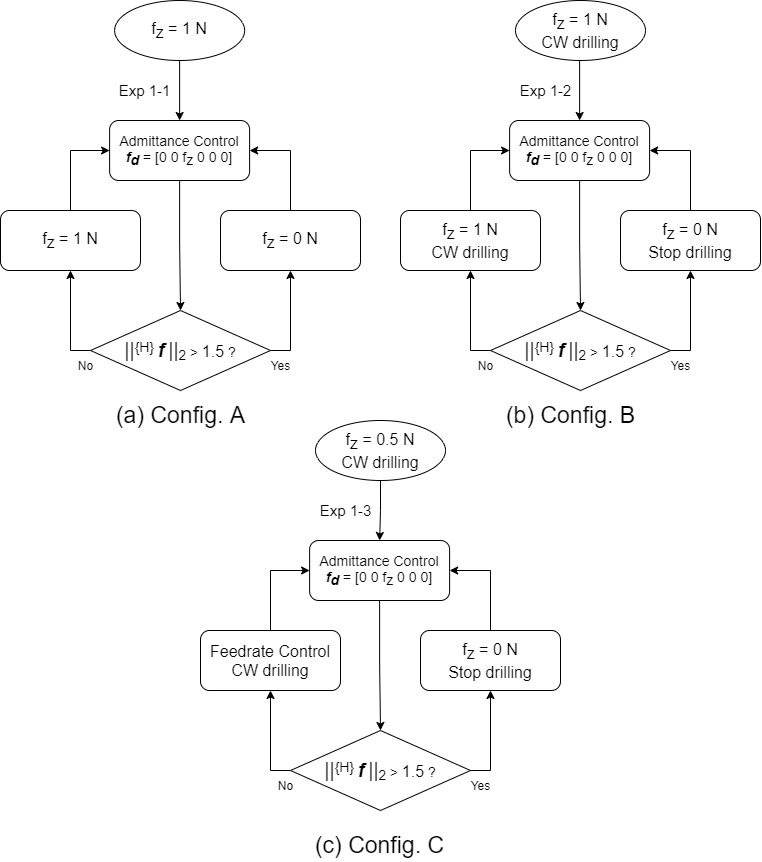
\includegraphics[width=1\linewidth]{Images/Exp1_motion planning.png}
\caption{Flow charts for force-guided alignment experiment}
\label{fig:exp_motion planning}
\end{center}
\end{figure}	

\begin{enumerate}
\item[1.1] Inserting without file rotation
\item[1.2] Inserting with file rotation
\item[1.3] Inserting with file rotation and file feedrate control
\end{enumerate}
\par
To simulate a patient moving, a Stewart platform with six degrees of freedom was incorporated.  When the patient moved to a point, our system should move to the same place. Therefore, the target's and the handpiece's positions should be compared to check if our system tracked the patient or not. PhaseSpace - Impulse X2E was involved in obtaining the above positions in real-time. 
\par
The Stewart platform is scheduled for motion planning. It will move to (0, 0, 0), (15, 0, 0), (15, 0, 15), (0, 0, 15) related to Stewart frame with a constant velocity. These points formed a square composed of two horizontal and two vertical lines. The command position trajectory is illustrated in Fig \ref{fig: position command}. The Stewart platform is planned to go along with the square with a velocity, then stop for $10$ seconds, then go along with the square with a faster velocity, and so on. The velocities of four rounds are $3$ mm/s, $4$ mm/s, $5$ mm/s, and $6$ mm/s.
	
\begin{figure}[htbp]
\begin{center}
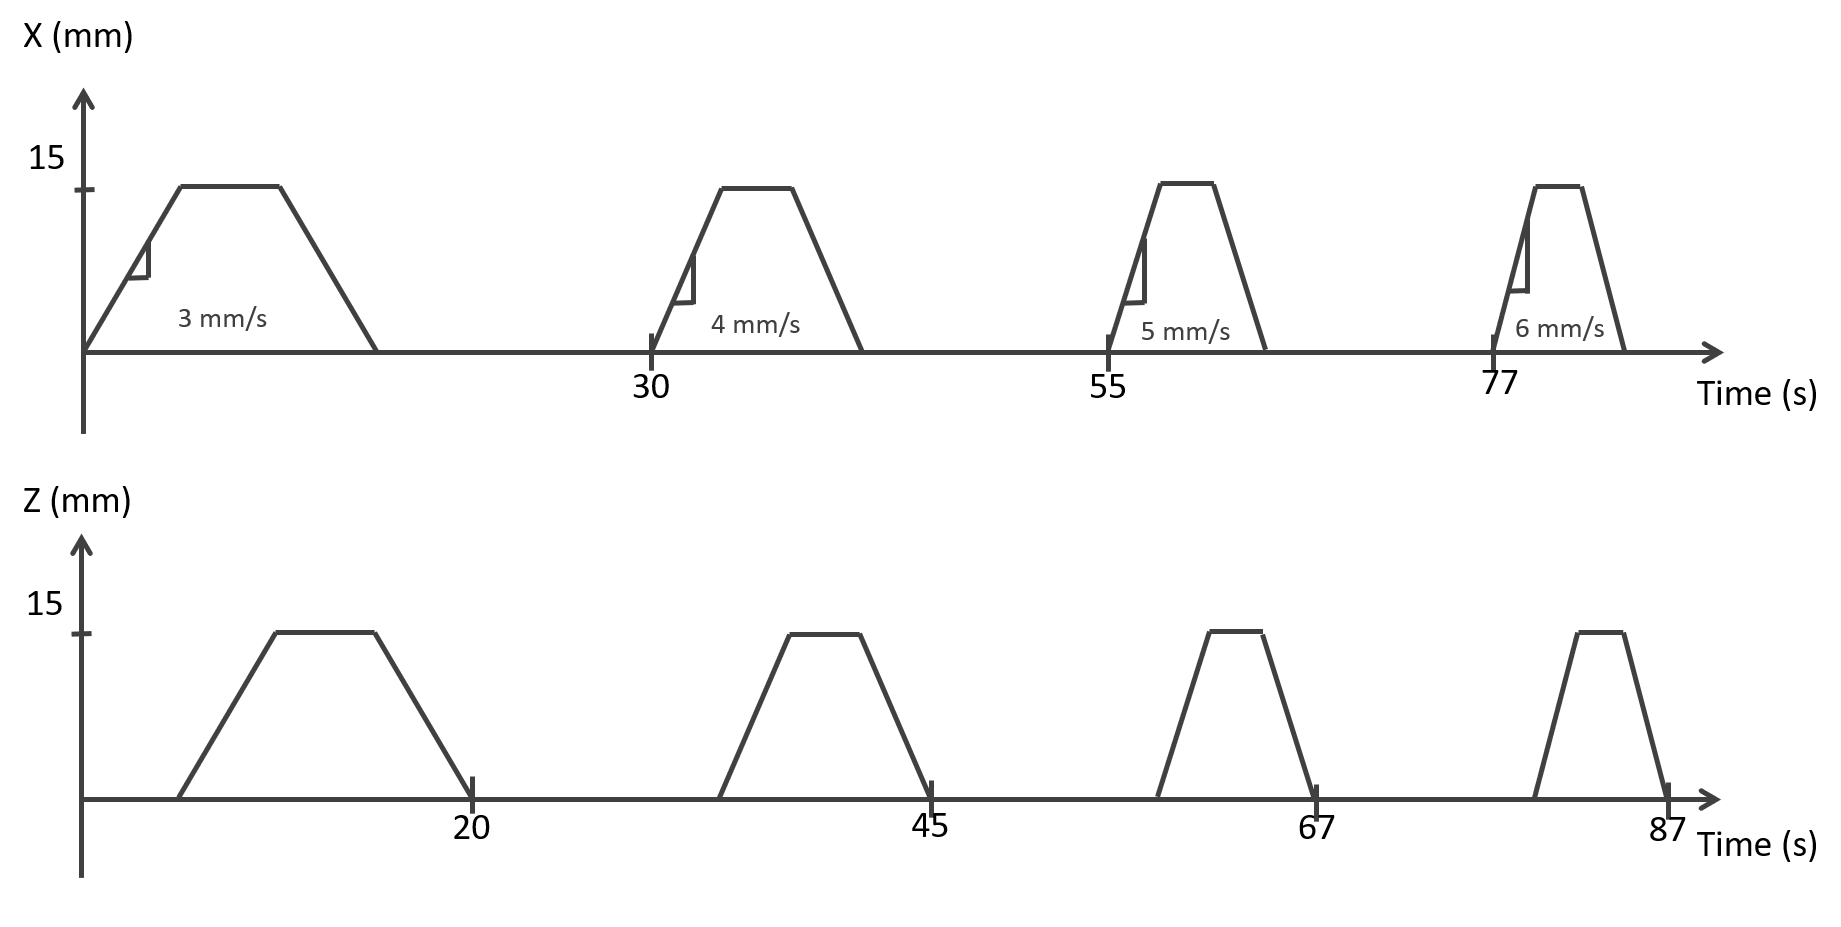
\includegraphics[width=1\linewidth]{Images/position command.png}
\caption{Position command of Stewart platform for force-guided alignment experiment}
\label{fig: position command}
\end{center}
\end{figure}	
\par
Parameters setting of admittance control in Experiment 1 was shown is Table \ref{tab: para_adm_exp1}. The parameter $\mathbf{K}$ was proportional to the gain and $\mathbf{B}$ was inversely proportional to the gain. Therefore, the same values were set in all experiment expect $b_6$. $b_6$ was relevant to the rotation along with z-axis. The rotation along with z-axis driven by the robot arm should be deactivated in Exp 1-1 and 1-2 because the file rotation was driven by the motor. If the rotation along with z-axis was on duty and the file was drilling, the robot arm would rotate along with z-axis in opposite direction. A slow inserting is required when performing the endodontic treatment. Therefore, The maximum value of $f_z$ was set $0.5$ in Exp 1-3 to limit the the highest velocity. Note that, the root acrylic model had drilled thoroughly by a file and formed a cone shape in advance.
\par
\begin{table}[htbp]
\centering
\tabcolsep=25pt
\caption{Parameters setting of admittance control in Experiment 1.}
\label{tab: para_adm_exp1}
\begin{tabular}{cccc} 
\hline \hline
Parameter	&Exp 1-1		&Exp 1-2		&Exp 1-3	\\
\hline
$k$			&$500$		&$500$		&$500$				\\
$f_z$		&$1$		&$1$		&$-0.2 \sim 0.5$	\\
$b_1$		&$80$		&$80$		&$80$				\\
$b_2$		&$80$		&$80$		&$80$				\\
$b_3$		&$80$		&$80$		&$80$				\\
$b_4$		&$80$		&$80$		&$80$				\\
$b_5$		&$80$		&$80$		&$80$				\\
$b_6$		&$80$		&$\infty$	&$\infty$			\\
\hline
\multicolumn{4}{c}{ $\mathbf{K} = \text{diag}(k,k,k,k,k,k), \mathbf{B} = \text{diag}(b_1,b_2,b_3,b_4,b_5,b_6)$} \\
\hline\hline	
\end{tabular}
\end{table}
\subsubsection{Result}
\hspace*{6mm} There were three metric types of figures to show the results of Exp 1-1, 1-2, and 1-3. An imperative metric was whether the robot could move as the root move. Therefore, the first figure was the position information. The position of robot and root were compared and the relative distance between them was evaluated. The left y-axis of the first figure was for the position of robot and root and the right one was for the relative distance. Second, the input of admittance control was force vector and output was velocity vector. Hence, the force and the velocity were compared in the second figure. Last, the force and the position of robot were compared in the third figure. Note that the real position and velocity data were transformed from the PhaseSpace frame to the Stewart platform frame. The force information were also transformed to the Stewart platform frame from the handpiece frame.

\begin{figure}[htbp]
\begin{center}
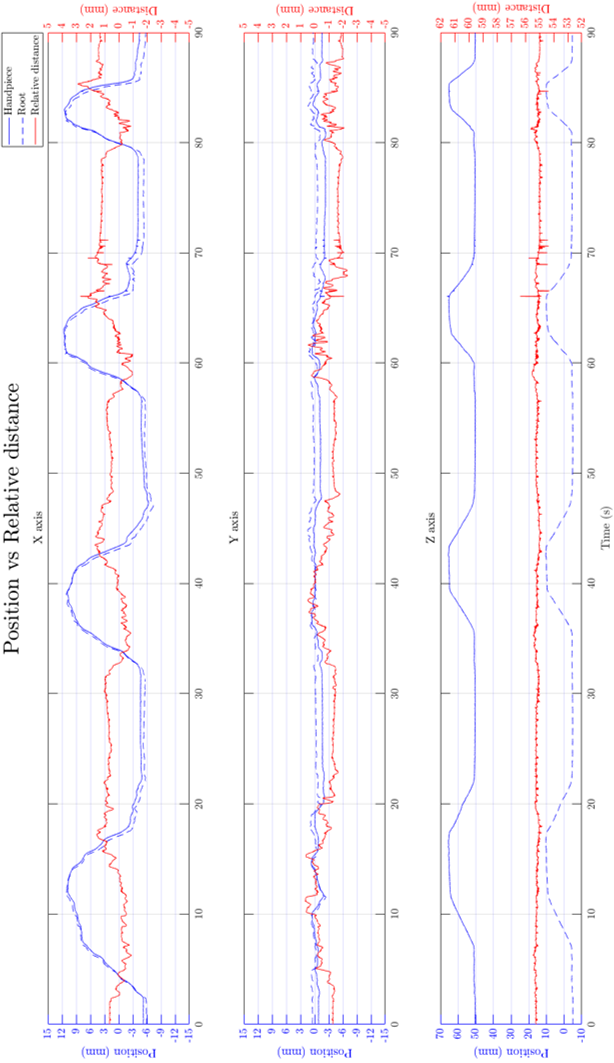
\includegraphics[width=1\linewidth]{Images/exp/exp1_1_1.png}
\caption{Exp 1-1: The position of robot and root and their relative distance}
\label{fig: exp1_1_1}
\end{center}
\end{figure}	
\begin{figure}[htbp]
\begin{center}
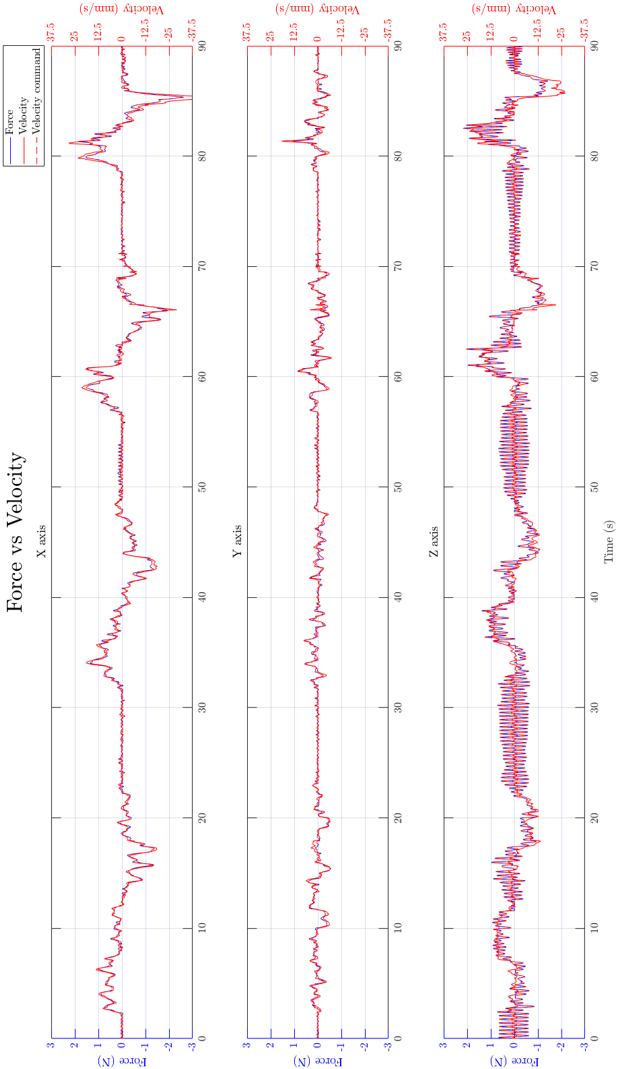
\includegraphics[width=1\linewidth]{Images/exp/exp1_1_2.png}
\caption{Exp 1-1: The force vs the velocity}
\label{fig: exp1_1_2}
\end{center}
\end{figure}	
\begin{figure}[htbp]
\begin{center}
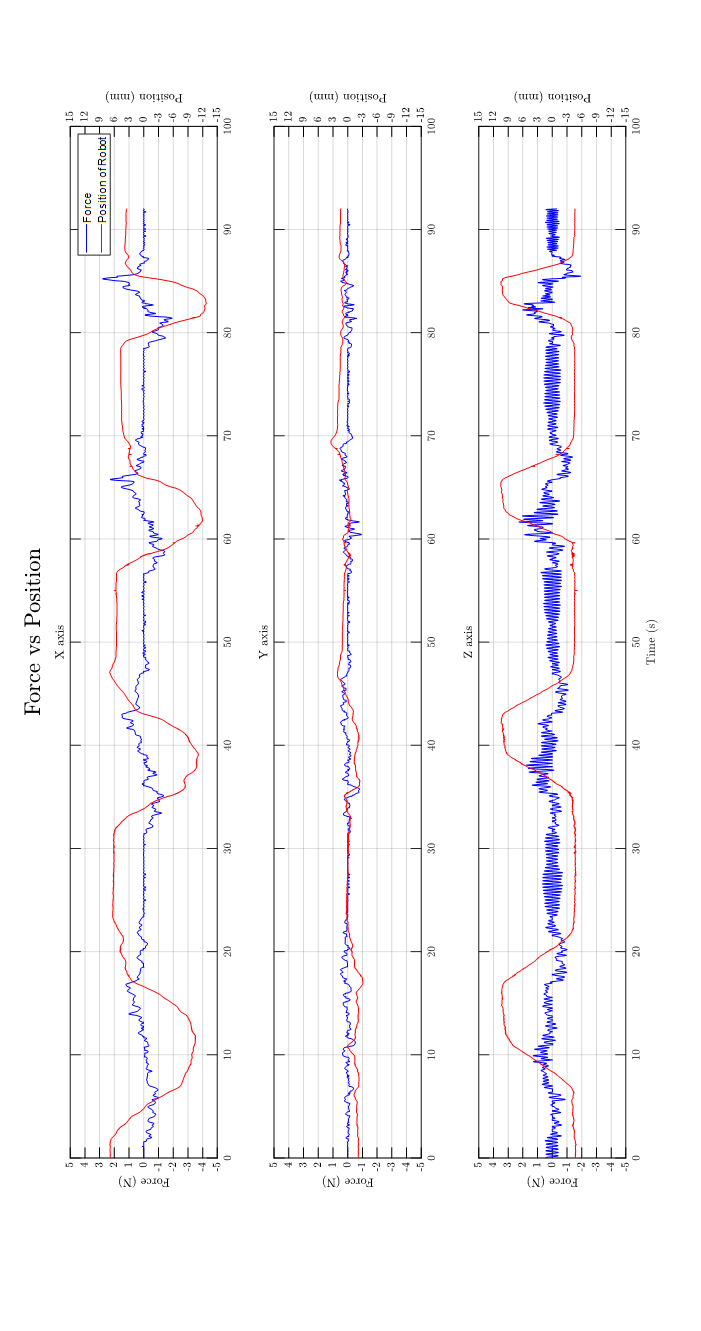
\includegraphics[width=1\linewidth]{Images/exp/exp1_1_3.png}
\caption{Exp 1-1: The force vs the position}
\label{fig: exp1_1_3}
\end{center}
\end{figure}	
\begin{figure}[htbp]
\begin{center}
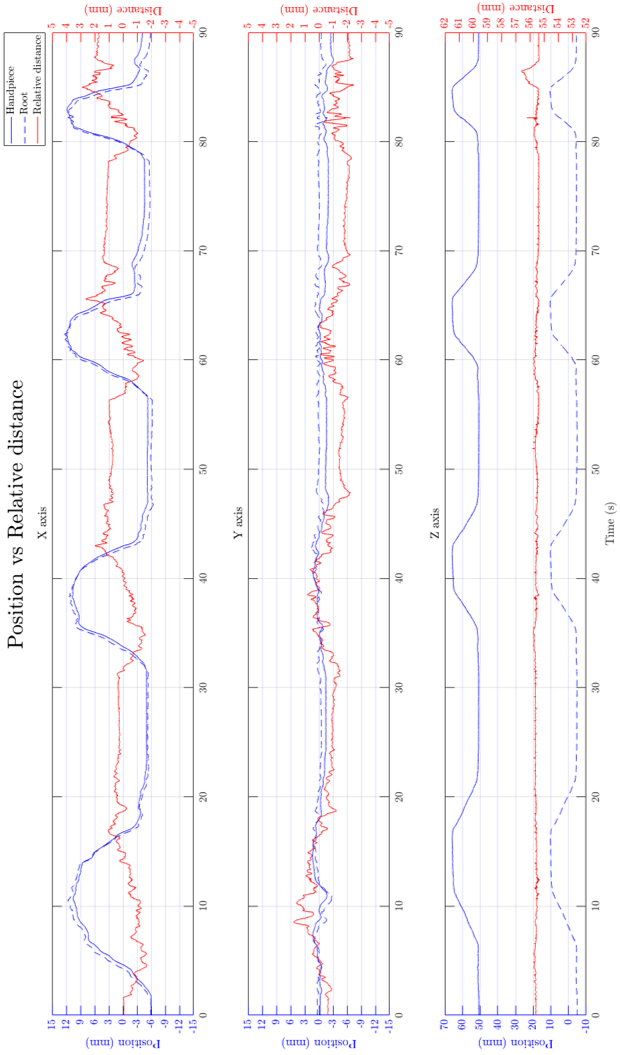
\includegraphics[width=1\linewidth]{Images/exp/exp1_2_1.png}
\caption{Exp 1-2: The position of robot and root and their relative distance}
\label{fig: exp1_2_1}
\end{center}
\end{figure}	
\begin{figure}[htbp]
\begin{center}
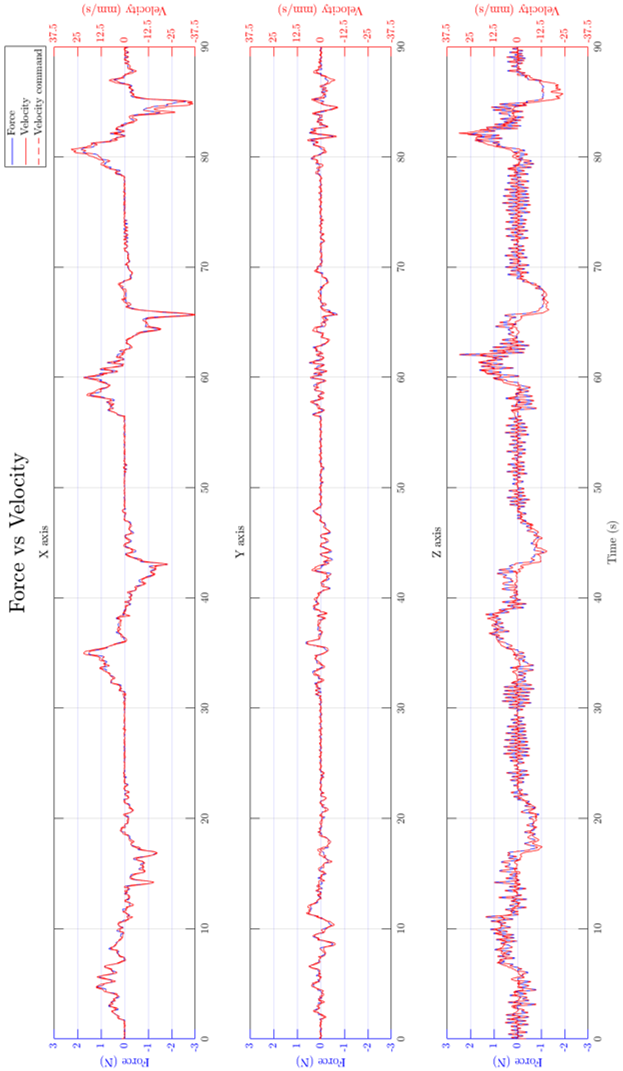
\includegraphics[width=1\linewidth]{Images/exp/exp1_2_2.png}
\caption{Exp 1-2: The force vs the velocity}
\label{fig: exp1_2_2}
\end{center}
\end{figure}	
\begin{figure}[htbp]
\begin{center}
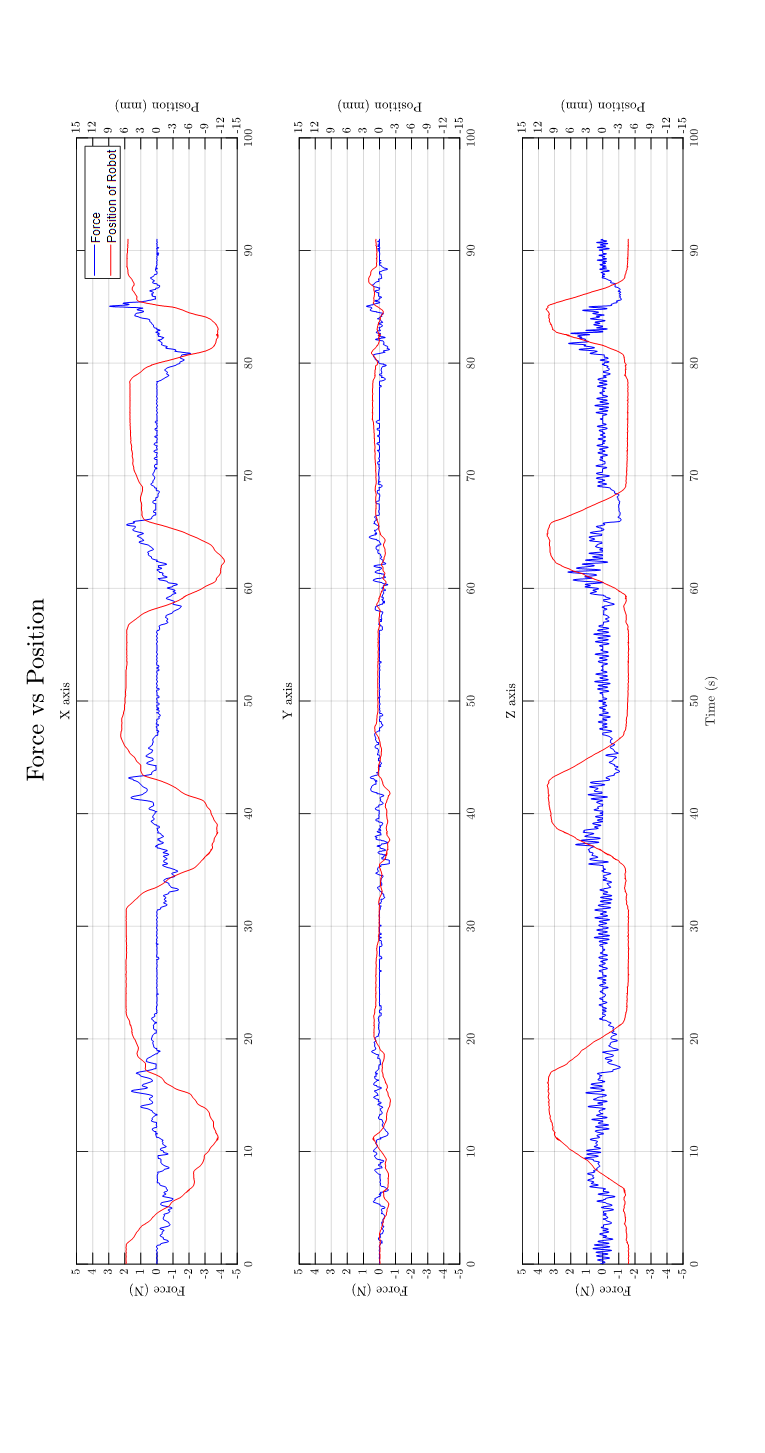
\includegraphics[width=1\linewidth]{Images/exp/exp1_2_3.png}
\caption{Exp 1-2: The force vs the position}
\label{fig: exp1_2_3}
\end{center}
\end{figure}	
\begin{figure}[htbp]
\begin{center}
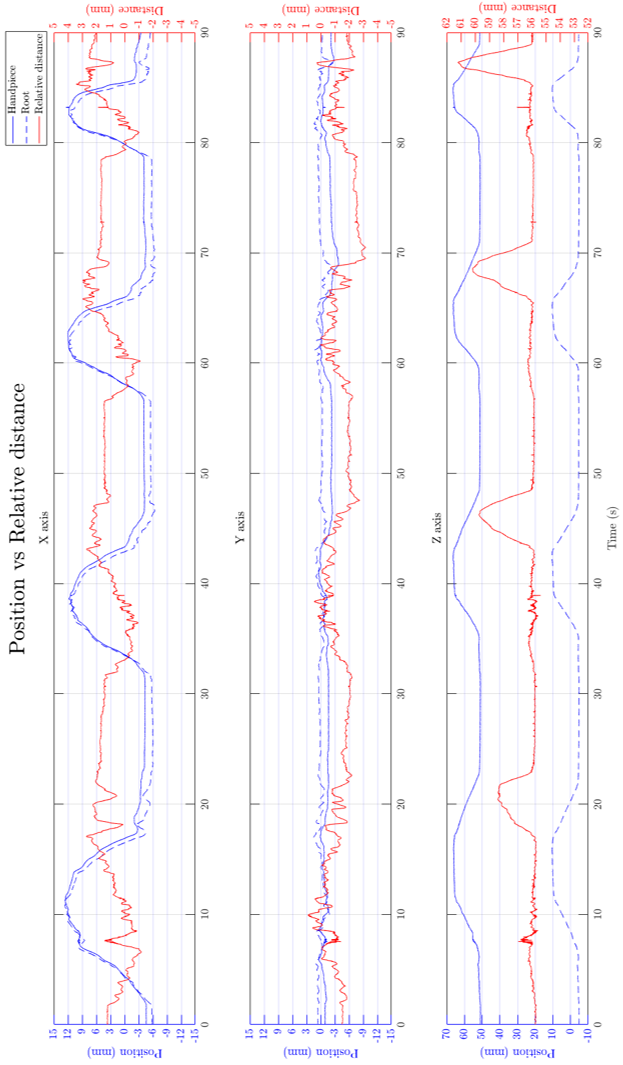
\includegraphics[width=1\linewidth]{Images/exp/exp1_3_1.png}
\caption{Exp 1-3: The position of robot and root and their relative distance}
\label{fig: exp1_3_1}
\end{center}
\end{figure}	
\begin{figure}[htbp]
\begin{center}
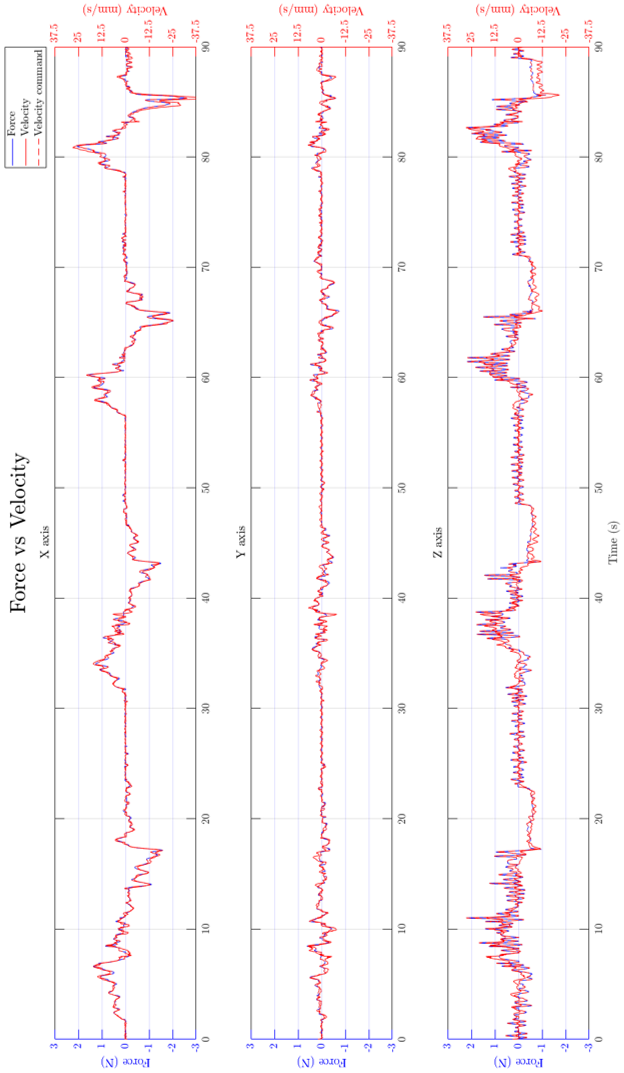
\includegraphics[width=1\linewidth]{Images/exp/exp1_3_2.png}
\caption{Exp 1-3: The force vs the velocity}
\label{fig: exp1_3_2}
\end{center}
\end{figure}	
\begin{figure}[htbp]
\begin{center}
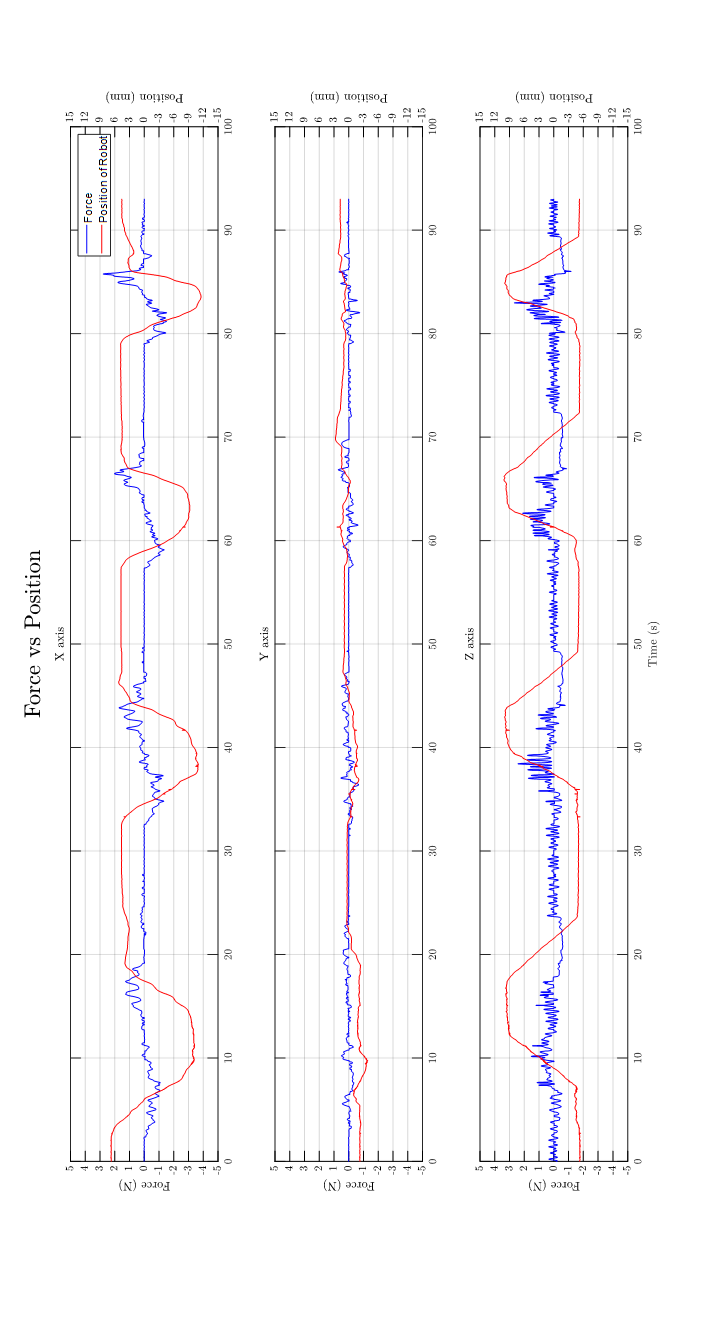
\includegraphics[width=1\linewidth]{Images/exp/exp1_3_3.png}
\caption{Exp 1-3: The force vs the position}
\label{fig: exp1_3_3}
\end{center}
\end{figure}	

\newpage

\section{Pre-Clinical Evaluation}
\hspace*{6mm}We have verified that it is feasible to apply parts of our proposed technical approaches in experiment 1. In what follows, an algorithm that combines all functions including force-guided alignment, inverse rotation control, and feed control were implemented in the pre-clinical trial as shown in Fig \ref{fig: exp2_motion planning}.
\begin{figure}[htbp]
\begin{center}
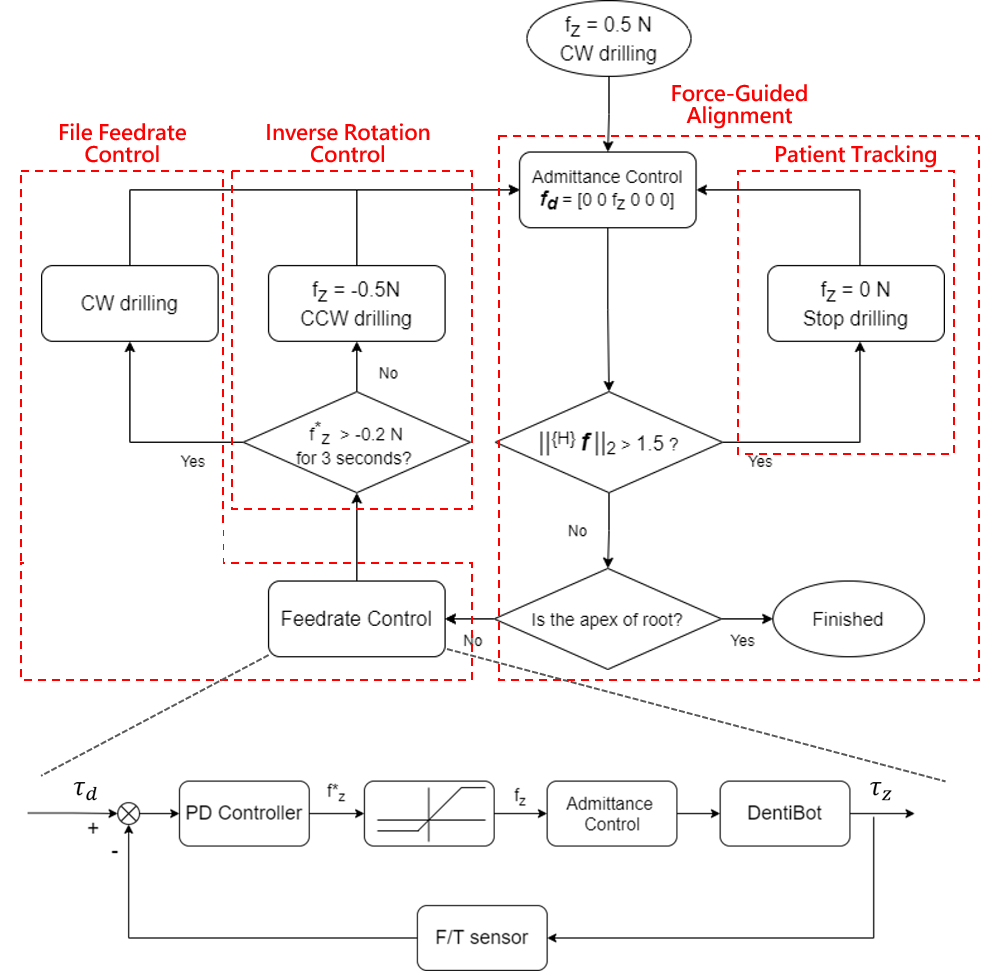
\includegraphics[width=1\linewidth]{Images/algorithm.png}
\end{center}
\caption{
Algorithm for robot-assisted endodontic treatment
}\label{fig: exp2_motion planning}
\end{figure}
\par
The metrics of the pre-clinical trial were completeness of root preparation and whether instrument fracture happened.
(Completeness definition: comparison of pixel area before and after experiment via image)
validation of repetitive experiment

\begin{figure}[htbp]
\begin{center}
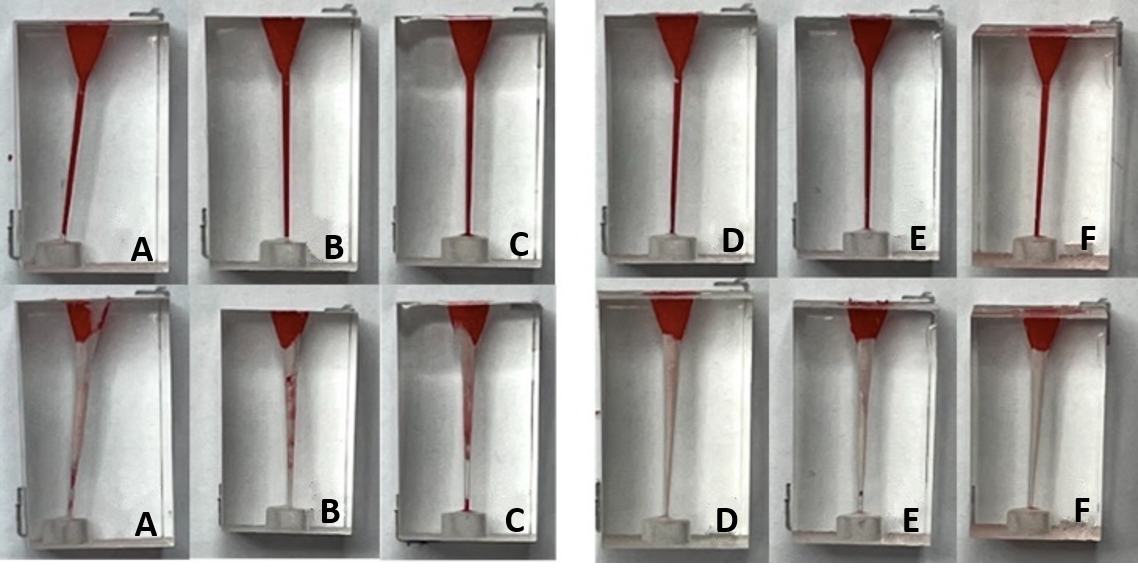
\includegraphics[width=1\linewidth]{Images/exp/roots.png}
\caption{Exp 2: Roots before and after drilling for two times. $T_{des}$ were set 40 in A,B,C and 50 in D,E,F}
\label{fig: exp2_roots}
\end{center}
\end{figure}	

\begin{figure}[htbp]
\begin{center}
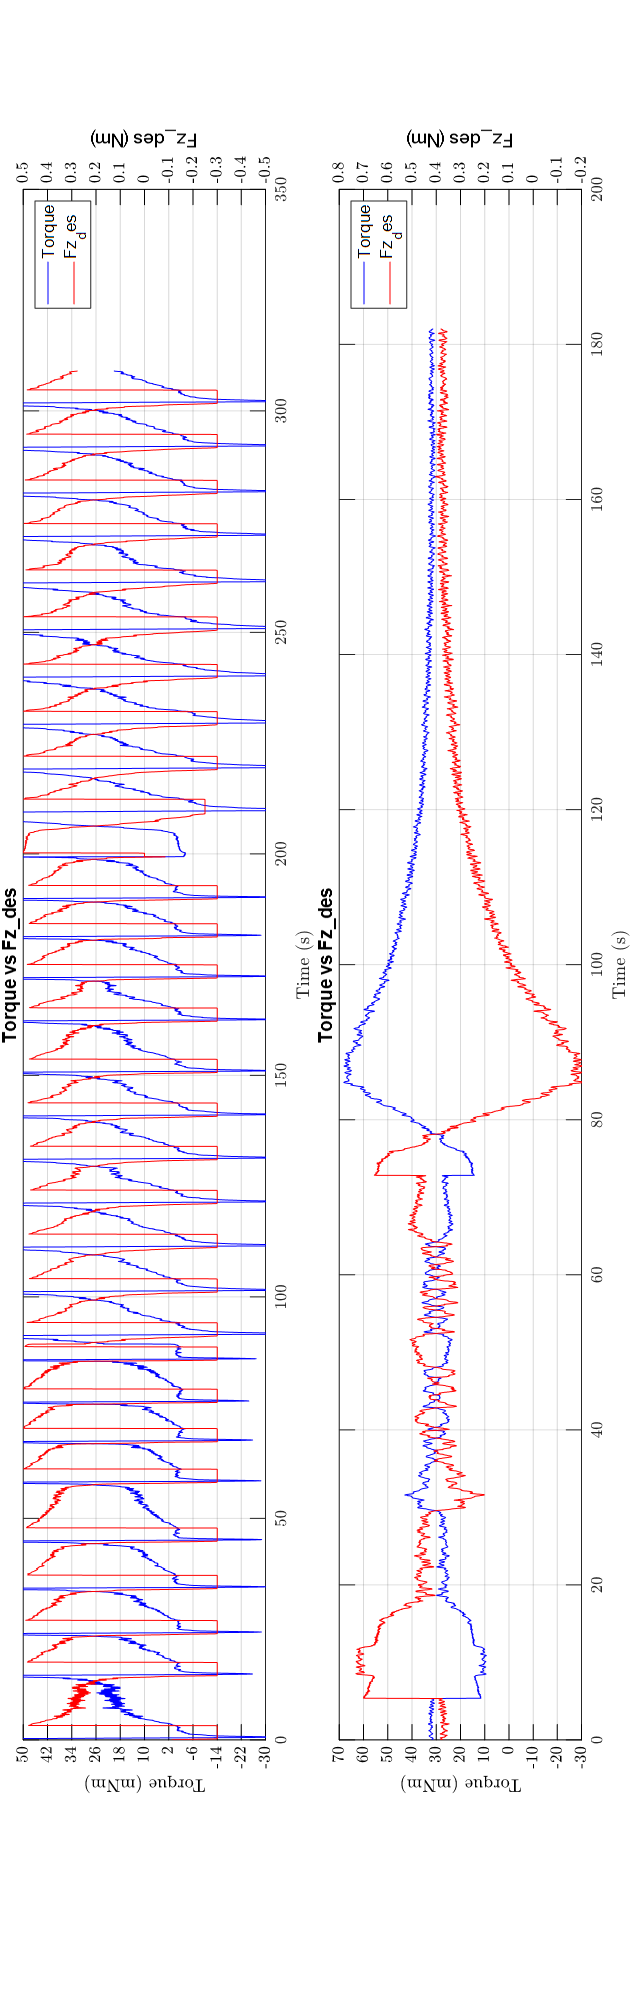
\includegraphics[width=1\linewidth]{Images/exp/exp2_torque.png}
\caption{Exp 2: The torque measured by F/T sensor and $f_z$}
\label{fig: exp2_torque}
\end{center}
\end{figure}	
 In this experiment, the performance of root preparation using our robot was demonstrated. 